\documentclass[11pt,a4paper]{scrartcl}
\typearea{12}
\usepackage{graphicx}
\usepackage{pstricks}
\usepackage{listings}
\lstset{language=C}
\pagestyle{headings}
\markright{COMS11600 - Principles of programming I.2}
\begin{document}

\subsection*{I.3 A quick note on the Travelling Salesperson Problem}

We have seen a linear, $O(n)$ algorithm, linear search and a
quadratic, $O(n^2)$, algorithm: insert sort. The running time of these
problems comes from having to go through the $n$ data items one-by-one
in the case of linear search, or, going through them one-by-one and
for each, having to go through the list of already sorted data. We
also looked at binary search which is an $O(\log{n})$ algorithm and
saw how the run time came from dividing the data in two at each
step. We will see a $O(c^n)$ algorithm soon. Here, we will look at why
an algorithm might be order $O(n!)$; basically a $O(n!)$ algorithm is
one that requires looking at every possible combination of something,
obviously for even modest values of $n$ the growth of $n!$ will make
the algorithm impractical.

Here, we'll look at the Travelling Salesperson Problem; the problem of
finding the shortest path joining a set of points. This is an old
problem, the Irish mathematician William Hamilton worked on it for
example, it is frequently used as an example in computational
complexity theory. In the \lq{}saleperson\rq{} description, imagine a
salesperson who wants to visit a collection of towns; what is the
ideal route this salesperson should take to minimize their path. There
is an algorithm which runs in $O(n^22^n)$, this is very slow, but much
better than the most obvious algorithm, checking each route,
calculating its length and then looking to see which is shortest. This is what is called a brute force approach.

To work out the number of paths, there are $n$ possible choices of
first town, followed by $n-1$ possible choices for second since one
has already been picked, $n-2$ possible for third, $n-3$ for fourth
and so on. This means the number of ways of designing a route by
putting the towns in the order they are to be visited is
$n(n-1)(n-2)\ldots 1=n!$. Now the direction of the route doesn't
effect its length, for example, if the towns are $A$, $B$ and $C$,
$ABC$ and $CBA$ are the same distance, just travelled in opposite
directions. However, the only effect this has is to halve the number
combinations, it leaves the algorithm $O(n!)$ even before including
the time it takes to work out the path length for each combination.

\begin{figure}
\begin{center}
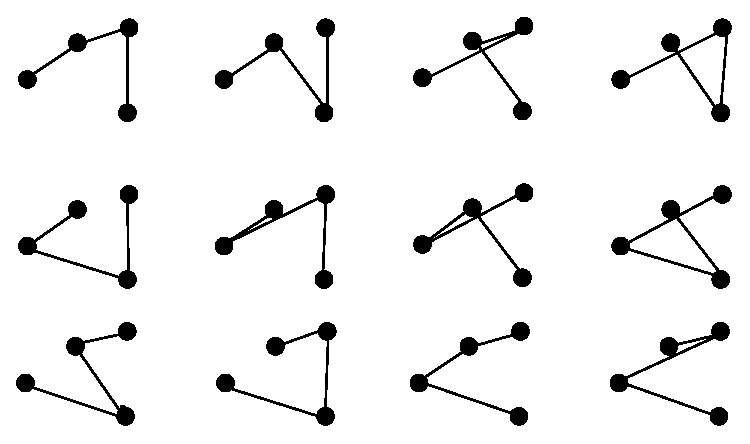
\includegraphics{travelling_sales.eps}
\end{center}
\caption{Here are the $4!/2=12$ paths which need to be computed and compared to solve the $n=4$ Travelling Salesperson Problem.}
\end{figure}

\end{document}
